\documentclass[10pt]{extarticle}
\title{Computer Science 2 Notes}
\author{Giacomo Ellero}
\date{Semester 2, 2023/2024}

\usepackage{amsfonts}
\usepackage{amsthm}
\usepackage{amssymb}
\usepackage{amsmath}
\usepackage{mathtools}
\usepackage{commath}
\usepackage{dirtytalk}
\usepackage{parskip}
\usepackage{mathrsfs}
\usepackage[many]{tcolorbox}
\usepackage{xparse}
\usepackage[a4paper,margin=1.5cm]{geometry}
\usepackage{bookmark}
\usepackage{bytefield}
\usepackage{minted}
\usepackage{capt-of}
\usepackage{float}
\usepackage{tikz}
\usepackage{enumitem}

\newcommand{\C}{\mathbb{C}}
\newcommand{\R}{\mathbb{R}}
\newcommand{\N}{\mathbb{N}}
\newcommand{\F}{\mathcal{F}}
\renewcommand{\Re}{\operatorname{Re}}
\renewcommand{\Im}{\operatorname{Im}}

\newenvironment{absolutelynopagebreak}
  {\par\nobreak\vfil\penalty0\vfilneg
   \vtop\bgroup}
  {\par\xdef\tpd{\the\prevdepth}\egroup
   \prevdepth=\tpd}

\newtcolorbox{examplebox}[1]{colback=green!5!white,colframe=green!40!black,title={#1},fonttitle=\bfseries,parbox=false}
\newtcolorbox{notebox}[1]{colback=blue!5!white,colframe=blue!40!black,title={Note: #1},fonttitle=\bfseries,parbox=false}
\newtcolorbox{bluebox}[1]{colback=blue!5!white,colframe=blue!40!black,title={#1},fonttitle=\bfseries,parbox=false}
\newtcolorbox{warningbox}[1]{colback=orange!5!white,colframe=orange!90!black,title={Warning: #1},fonttitle=\bfseries,parbox=false}
   
\begin{document}

\maketitle
\tableofcontents
\clearpage

\section{Class of 06/02/2024}

\subsection{Asymptotic notation}

\begin{bluebox}{Definition}
    If $\exists C \in \R^+$ and $N \in \N$ such that for two sequences $a_n, b_n > 0$
    we have that $a_n \leq Cb_n$ for all $n \geq N$, then we write $a_n = O(b_n)$ and we read \say{$a_n$ is big O of $b_n$}.
\end{bluebox}

These sequences describe the time it takes for an algorithm to solve a certain problem of size $n$.

\begin{examplebox}{Example}
    Let $a_n = n^2 + 2n + 1$. We will prove that $a_n = O(n^2)$.

    \begin{proof}
        We have that
        \begin{align*}
            a_n & = n^2 + 2n + 1        \\
                & \leq n^2 + 2n^2 + n^2 \\
                & = 4n^2
        \end{align*}
    \end{proof}

    As we can see just need to show that $C$ exists, we don't need to find the best one.
\end{examplebox}

Usually we don't use limits to prove that a sequence is big O of another, it is usually more convenient to proceed by inequalities.

\begin{notebox}{Logarithms}
    When we have sequences with logarithms we don't need to specify the basis,
    as the logarithm is a constant factor of another logarithm by the change of basis formula.
\end{notebox}

\subsubsection{Operations and other notation}

Let $a_n = O(c_n)$ and $b_n = O(d_n)$, then we have that

\begin{itemize}
    \item $a_n + b_n = O(\max\{c_n, d_n\})$
    \item $a_n \cdot b_n = O(c_n \cdot d_n)$
\end{itemize}

We also define the \say {opposite} of big O notation, the $\Omega$ notation:
$a_n$ is $\Omega(b_n)$ if $a_n \geq Cb_n$ for all $n \geq N$.

Moreover, if $a_n = O(b_n)$ and $a_n = \Omega(b_n)$ (for some different $C$ and $N$) then we write $a_n = \Theta(b_n)$.

\subsection{Randomness}

When we run an experiment we can define
\begin{itemize}
    \item an outcome $\omega_i$
    \item the value of the outcome $x_i$ (similar to a bet)
    \item the probability of the outcome $p_i$
\end{itemize}

We can also define the expected result $E(X)$ of the experiment as
$$
    E(X) = \sum ^n _{i = 1} x_i p_i
$$

\subsection{IEEE-754}

This is not in the syllabus but it's useful to know.

IEEE-754 is a standard for representing floating point numbers in computers.
We will discuss in particular the 32-bits representation but larger or smaller formats also exist.

We subdivide the 32 bits in 3 parts: 1 bit for the \textbf{sign}, 8 bits for the \textbf{exponent}, and 23 bits for the \textbf{fraction} or mantissa.

\begin{center}
    \begin{bytefield}[bitwidth=1.1em, bitheight=\widthof{~Sign~}]{32}
        \bitheader{0,8,31} \\
        \bitbox{1}{1}
        \bitboxes{1}{00100101}
        \bitboxes{1}{00110110101101001111011} \\
        \bitbox{1}{\rotatebox{90}{Sign}}
        \bitbox{8}{Exponent}
        \bitbox{23}{Fraction}
    \end{bytefield}
\end{center}

The number is interpreted according to the following formula:

$$
    n = (-1)^s \cdot 2^{e - 127} \cdot (1 + f)
$$

Basically the number is represented in scientific notation, in base 2.

Note that when converting the fraction part to decimal the powers of 2 are negative and decreasing
(i.e.: bit at 9 is $2^{-1}$, bit at 10 is $2^{-2}$, etc).

\section{Class of 08/02/2024}

\subsection{Introductory statements}

We will start by stating the following facts without providing a proof (they can be proven but in class we skipped them).

\begin{itemize}
    \item If $c \in \R^+$, then $g(n) = 1 + c + c^2 + \dots + c^n$ is $\Theta(1)$ if $c < 1$, $\Theta(n)$ if $c = 1$, and $\Theta(c^n)$ if $c > 1$.
    \item In any base $b \ge 2$ the sum of any 3 single-digit numbers is at most 2 digits long.
    \item $\forall n \in \N$ and any base $b$ there exists a power of $b$ in $[n, bn].$
\end{itemize}

\begin{notebox}{$\Theta(1)$}
    When we say that a function is $\Theta(1)$ we mean that it is bounded from above by a constant $C$ (since it is big O of 1)
    and bounded from below by a constant $c$ (since it is $\Omega(1)$).

    This usually means that $a_n \ne 0$ for all $n$.
\end{notebox}

\subsection{How to approach a algorithm problem}

We usually proceed by following these steps:
\begin{enumerate}
    \item Find an algorithm
    \item Prove that the algorithm is correct
    \item Calculate the time complexity of the algorithm
          \begin{enumerate}
              \item Can we do better?
          \end{enumerate}
\end{enumerate}

We will use the following steps to approach some classic problems such as addition and multiplication of binary numbers.

\begin{notebox}{Shifts}
    We refer to shifts as the operation of moving all the bits of a number to the left or to the right by a certain amount of positions.
    This operation mathematically corresponds to multiplying or dividing the number by a power of the base.

    $$
        x \ll n = x \cdot b^n
    $$

    The $\ll$ symbol denotes a left shift by $n$ positions, while the $\gg$ symbol denotes a right shift by $n$ positions.

    In our mathematical world each shift is $O(n)$, in the real world it is usually $O(1)$.
\end{notebox}

\subsection{Addition}

\underline{Problem}: Let $x, y$ be binary numbers of $n$ bits. We want to compute $x + y$.

We proceed by using the normal addition algorithm: this is a well know algorithm that we know is correct.

At each step we are adding at most 3 numbers (2 bits and a carry).
We know that the result of each step is at most 2 bits long: one bit goes for the result and the other goes for the carry.
This ensures that at the next step we will also be adding at most 3 numbers, hence each step is performed in a finite amount of time.

Since we are performing $n$ steps, the time complexity of this algorithm is $O(n)$.

\textit{Can we do better?} No, we can't, since we need to read all the bits of the input and this operation is already $O(n)$.

\subsection{Multiplication}

\underline{Problem}: Let $x, y$ be binary numbers of $n$ bits. We want to compute $x \cdot y$.

Again, we proceed using the normal multiplication algorithm that we know is correct.
The algorithm has the following parts:
\begin{enumerate}
    \item Write the multiplications of $x$ by each bit of $y$
    \item Sum all the results
\end{enumerate}

\textbf{Part 1}: Let $(s_n)$ be the sequence of the shifted values of $x$ and $p_n$ be the sequence of the partial products.

\begin{align*}
    s_0 & = x                         \\
    s_n & = s_{n-1} \ll 1             \\
    p_n & = \begin{cases*}
                0   & \text{if } y[n] = 0 \\
                s_n & \text{if } y[n] = 1
            \end{cases*}
\end{align*}

Choosing the right $p_n$ is $O(1)$, but computing $s_n$ is $O(n)$ hence this part is $O(n)$.

Note that we are \say{storing} the result of the previous shifts, so if we want to compute $s_5$, for example, we don't need to compute $s_4$ again.
Without this optimization the time complexity of this part would be $O(n^2)$.

\textbf{Part 2}:
In this step we are computing $\sum_{i = 0}^n p_n$.
These are sums of numbers of at most $2n$ bits, hence this part is $O(n)$.

\textbf{Conclusion}: The time complexity of the multiplication algorithm is $O(n) \cdot O(n) = O(n^2)$.

\subsubsection{Egyptian Multiplication}

This is an ancient algorithm that is used to multiply two numbers.
It works as follows:

\begin{enumerate}
    \item Write the two numbers in two columns
    \item Divide the first number by 2, floor the result and write it underneath it in the same column
    \item Multiply the second number by 2 and write the result underneath it in the same column
    \item When the first number is 1, sum all the numbers in the second column if the corresponding number in the first column is odd
\end{enumerate}

We can easily implement this algorithm in Python as follows:
\begin{minted}{python}
    def egyptian_multiplication(x, y):
        result = 0
        while x >= 1:       # This loop runs n times since x has n bits
            if x % 2 == 1:  # We always consider the worst case, hence this is always true
                result += y # Sums are O(n)
            x = x >> 2      # Shifts are O(n)
            y = y << 2      # Shifts are O(n)
        return result
\end{minted}

The complexity of the algorithm is $(O(n) + O(n) + O(n)) \cdot O(n) = O(n^2)$.

\subsubsection{Other multiplication algorithms}

Another algorithm we can use to implement multiplication works by dividing each number in half and recursively computing the result.

First we write the two numbers as
\begin{align*}
    x & = 2^{\frac{n}{2}}x_{\text{up}} + y_{\text{low}} \\
    y & = 2^{\frac{n}{2}}y_{\text{up}} + y_{\text{low}}
\end{align*}

Where $x_{\text{up}}$ and $y_{\text{up}}$ are the upper halves of $x$ and $y$ and $x_{\text{low}}$ and $y_{\text{low}}$ are the lower halves of $x$ and $y$.

Then we compute the result as
$$
    x \cdot y = 2^n x_{\text{up}}y_{\text{up}} + 2^{\frac{n}{2}}(x_{\text{up}}y_{\text{low}} + x_{\text{low}}y_{\text{up}}) + x_{\text{low}}y_{\text{low}}
$$

Each time we are performing 4 multiplication of half the size and adding them together.
The time this algorithm takes is
$$
    T(n) = 4T\left(\frac{n}{2}\right) + O(n)
$$

However if we keep expanding the recursion we will see that eventually we get to $T(1)$ which is $O(1)$
and we are left with $n$-many $O(n)$ terms, hence the time complexity of this algorithm is also $O(n^2)$.

\section{Class of 09/02/2024 - Divide and Conquer}

In this class we will see a class of algorithm that
split the problem in smaller sub-problems which are easier to compute and then combine the results.

\subsection{Karatsuba's algorithm}

This is a multiplication algorithm that is based on the last algorithm we discussed in the last class with some variations.

The algorithm takes inspiration from the multiplication of two complex numbers:
\begin{align*}
    (a + bi)(c + di) & = (ac - bd) + (ad + bc)i   \\
    \implies bc + ad & = (a + b)(c + d) - ac - bd
\end{align*}

Applying this to the multiplication of two binary numbers we get
\begin{align*}
    x \cdot y & = x_{\text{up}} y_{\text{up}} 2^n
    + 2^\frac{n}{2}((x_{\text{up}} + x_{\text{low}})(y_{\text{up}} + y_{\text{low}}) - x_{\text{up}}y_{\text{up}} - x_{\text{low}}y_{\text{low}}) + x_{\text{low}}y_{\text{low}}
\end{align*}

By doing this we are performing 3 multiplications of half the size and 4 additions.
Since we saw how additions are faster than multiplications we can expect this algorithm to be faster than the previous one.

$$
    T(n) = 3T\left(\frac{n}{2}\right) + O(n)
$$

We can arrange the work in nodes of a tree:

\begin{center}
    \begin{tabular}{ |c|c|c|c| }
        \hline
        level  & nodes  & work per node    & total work                      \\
        \hline
        0      & 1      & $Cn$             & $Cn$                            \\
        1      & 3      & $\frac{n}{2}C$   & $\frac{3}{2}Cn$                 \\
        2      & 9      & $\frac{n}{4}C$   & $\frac{9}{4}Cn$                 \\
        \vdots & \vdots & \vdots           & \vdots                          \\
        $k$    & $3^k$  & $\frac{n}{2^k}C$ & $\left(\frac{3}{2}\right)^k Cn$ \\
        \hline
    \end{tabular}
\end{center}

We have that the total work is the sum of the total work at each level of the tree:
$$
    Cn\left(1+\frac{3}{2}+\left(\frac{3}{2}\right)^2+\dots+\left(\frac{3}{2}\right)^k\right)
$$

Compared to the \say{old} algorithm that has a total work that looks like

$$
    Cn\left(1+2+2^2+\dots+2^k\right)
$$

Through some algebra we can show that this sum is $3Cn^{\log_{2}3}$,
hence proving that the algorithm is $O(n^{\log_{2}3}) \sim O(n^{1.58})$.

\subsection{The master theorem}

This theorem helps us to compute the time complexity of divide and conquer algorithms.
The proof of the theorem is quite complex and, despite being written here, it is not as important as understanding the statement.

\underline{Statement}: If $a > 0, b > 1, d \ge 0$, $n$ is a power of $b$, and
$T(n)$ is defined by induction as
\begin{align*}
    T(1) & = 1                                   \\
    T(n) & = aT\left(\frac{n}{b}\right) + O(n^d)
\end{align*}

Where
\begin{itemize}
    \item $a$ is the number of subproblems
    \item $b$ is the factor by which the problem size is reduced at each step
    \item $d$ is the exponent in the work done at each level
\end{itemize}

Then

\begin{align*}
    T(n) = \begin{cases}
               O(n^d)          & \text{if } d > \log_b a \\
               O(n^d \log n)   & \text{if } d = \log_b a \\
               O(n^{\log_b a}) & \text{if } d < \log_b a
           \end{cases}
\end{align*}

\begin{proof}
    We can write a table with the work to be done at each size of the problem

    \begin{center}
        \begin{tabular}{ |c|c|c|c| }
            \hline
            level  & \# of problems & size of each problem & total work                         \\
            \hline
            0      & 1              & $n$                  & $Cn^d$                             \\
            1      & $a$            & $\frac{n}{b}$        & $Ca\left(\frac{n}{b}\right)^d$     \\
            2      & $a^2$          & $\frac{n}{b^2}$      & $Ca^2\left(\frac{n}{b^2}\right)^d$ \\
            \vdots & \vdots         & \vdots               & \vdots                             \\
            $k$    & $a^k$          & $\frac{n}{b^k}$      & $Ca^k\left(\frac{n}{b^k}\right)^d$ \\
            \hline
        \end{tabular}
    \end{center}

    with $k = \log_b n$.

    To find the total work we need to sum all the total work at each step.
    With some algebra we can show that the total work is
    $$
        Cn^d\left(1+\left(\frac{a}{b^d}\right)+\left(\frac{a}{b^d}\right)^2+\dots+\left(\frac{a}{b^d}\right)^k\right)
    $$

    We can consider the following 3 cases:
    \begin{itemize}
        \item If $\frac{a}{b^d} = 1$, then $d = \log_b a$ and the sum becomes $ ??? $ and its complexity is $O(n^d \log n)$
        \item If $\frac{a}{b^d} < 1$, then $d > \log_b a$ and the sum becomes $ ??? $ and its complexity is $O(n^d)$
        \item If $\frac{a}{b^d} > 1$, then $d < \log_b a$ and the sum becomes $ ??? $ and its complexity is $O(n^{\log_b a})$
    \end{itemize}

    % TODO: complete the proof with picture and book
\end{proof}

\subsection{Introduction to sorting algorithms}

\subsubsection{Comparison based sorting}

Every comparison-based sorting algorithm
must do $\Omega(n \log n)$ comparison to sort $n$ distinct elements in the worst case.

\underline{Statement}: For any comparison-based algorithm $A$, for all $n \ge 2$ there exists an input of size $n$
such that $A$ makes at least $\log_2(n!) = \Omega(n \log n)$ comparisons.

The $n!$ comes from the fact that the factorial represents all the possible permutations of $n$ numbers,
hence, when we are sorting, we are just finding the \say{correct} permutation that sorts the input.

The $\log_2$ comes from the fact that each comparison we are making a choice, which the end gives two outcomes,
each one with half the options available for the next permutation.
Since we are looking for the worst outcome we have that we stop after $\log_2$ of the number we started with.

\subsubsection{Sorting without comparisons}

This is kinda surprising but it is actually possible if we have some other information about the input we are sorting.

For example, if we know that the input is a sequence of integers in a certain range we can use the \textbf{counting sort} algorithm.
This algorithm works by counting the occurrences of each number in the input and then writing them in the correct order.
This is a very fast algorithm compared to other generic sorting and takes $O(n)$ time.

Other examples of sorting algorithms that don't use comparisons are \textbf{radix sort} and \textbf{bucket sort}.

\subsection{Finding the median}

In general we can sort the list and find the median like that, which would be $O(n \log n)$.
It turns out that we can do better than that.

We will solve the more general problem that looks like this:
\begin{itemize}
    \item \textit{Input}: A list of numbers $S$; an integer $k$
    \item \textit{Output}: The $k$-th smallest element of $S$
\end{itemize}

In particular if $k = \frac{|S|}{2}$ we have that $k$ is the median.

\subsubsection{Description of the algorithm}

To do so we will use a recursion based algorithm:

\begin{enumerate}
    \item Select an element $V$ from $S$ at random
    \item We create 3 sub-lists:
          \begin{enumerate}
              \item $S_L = {x \in S : x < V}$
              \item $S_V = {x \in S : x = V}$
              \item $S_R = {x \in S : x > V}$
          \end{enumerate}
    \item We now call the algorithm recursively with the following parameters:
          \begin{enumerate}
              \item If $k \le |S_L|$ then we call the algorithm with $S_L$ and $k$
              \item If $|S_L| < k \leq |S_L| + |S_V|$ then we return $V$
              \item If $k > |S_L| + |S_V|$ then we call the algorithm with $S_R$ and $k - |S_L| - |S_V|$
          \end{enumerate}
\end{enumerate}

\subsubsection{The choice of V}

To calculate the time complexity of this algorithm we first have to choose a good $V$.
This is a hard task, because the \say{best} $V$ would be the median, but that's exactly what we are trying to find;
on the other hand the \say{worst} $V$ would be the minimum or the maximum of the input, which would reduce the problem size by only 1.

Since we cannot choose a good $V$ we will choose a random $V$:
the odds of choosing the best or the worst cases are both extremely unlikely,
hence we need to define a \say{good enough} $V$.

We consider a good enough $V$ if it lies between $\frac{1}{4}$ and $\frac{3}{4}$ of the input,
hence we can expect that the size of the sub-problems will be at most $\frac{3}{4}$ of the original problem.

This choice is arbitrarily, we could have chosen any other fraction and the time complexity,
as we will see later, would have been the same.
We chose these fractions because in this way the input
is divided in 2 \say{bad} cases of size $\frac{1}{4}$ and a \say{good} case of size $\frac{1}{2}$,
hence the size of the \say{bad} part is the same as the size of the \say{good} part.

\subsection{Time complexity}

We can now compute the time complexity

$$
    T(n) = \underbrace{T\left(\frac{3}{4}n\right)}
    _{\text{expected reduction}} +
    \underbrace{O(n)}_{\text{comparisons with } V}
    + \underbrace{\gamma O(n)}_{\text{finding a good } V}
$$

Note that $\gamma$ is the byproduct of the random choice of $V$,
we don't know how many times we will have to choose $V$ to find a good one.

Although we cannot be sure about the exact time this algorithm takes,
we can compute the \textbf{expected} time.

We saw before how the probability of choosing a good $V$ is $\frac{1}{2}$.
We can calculate the expected time as follows:
we pick a random $V$ and

\begin{enumerate}
    \item If $V$ is good we are done
    \item If $V$ is bad we need to repeat the algorithm
\end{enumerate}

Hence we have that $E = 1 + \frac{1}{2} E$, thus $E = 2$.
We have


\begin{align*}
    E(T(n)) & = E\left(T\left(\frac{3}{4}n\right)\right) + O(n) + 2O(n) \\
            & = O(n) + O(n) + 2O(n)                                     \\
            & = O(n)
\end{align*}

\begin{notebox}{Other solutions}
    This algorithm is presented to illustrate that algorithms that make use of random variables exist and can be useful;
    in the case of this specific problem there exist better algorithms that can solve the problem in a deterministic way,
    such as the \textbf{median of medians} algorithm.
\end{notebox}

\section{Class of 13/02/2024 - Graphs}

This week we will be working on graphs, this is referenced in chapter 3 of the book.

\begin{center}

    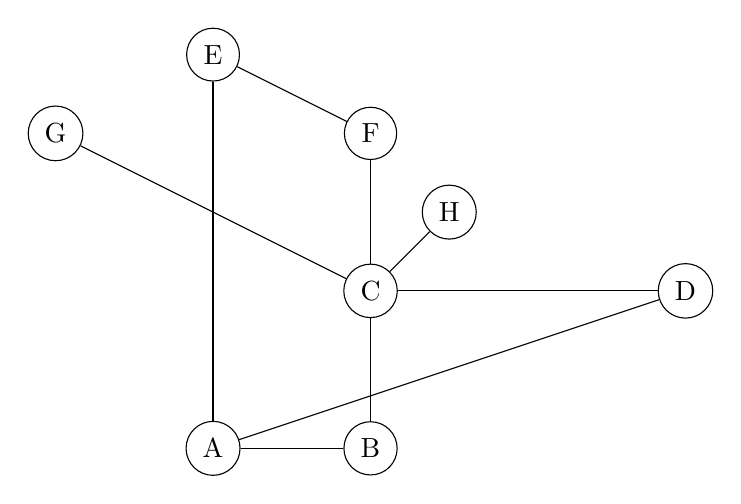
\begin{tikzpicture}
        \node[draw, circle] (A) at (0, 0) {A};
        \node[draw, circle] (B) at (2, 0) {B};
        \node[draw, circle] (C) at (2, 2) {C};
        \node[draw, circle] (D) at (6, 2) {D};
        \node[draw, circle] (E) at (0, 5) {E};
        \node[draw, circle] (F) at (2, 4) {F};
        \node[draw, circle] (G) at (-2, 4) {G};
        \node[draw, circle] (H) at (3, 3) {H};

        \draw (A) -- (B);
        \draw (B) -- (C);
        \draw (C) -- (D);
        \draw (D) -- (A);
        \draw (A) -- (E);
        \draw (E) -- (F);
        \draw (F) -- (C);
        \draw (C) -- (G);
        \draw (H) -- (C);
    \end{tikzpicture}
    \captionof{figure}{An example of a graph} \label{fig:graph}
\end{center}

Graphs can be useful to represent a lot of different things,
for example relationships, networks, maps, tournaments, etc.

\subsection{Definitions}

\begin{bluebox}{Definition}
    A \textbf{graphs} $G = (V, E)$ is a pair of finite sets where
    $V$ is the set of \textbf{vertices} (or nodes) and $E$ is the set of \textbf{edges}.

    $E$ is a subset of $V \times V$.
\end{bluebox}

The elements of $E$ are pairs of vertices that represent the connections between the vertices.

These are some other useful definitions we will use:
\begin{description}
    \item[Adjacent vertices] If $e = (u, v) \in E$ then we say that $u$ and $v$ are adjacent.
    \item[Incident edges] If $e = (u, v) \in E$ then we say that $e$ is incident to $u$ and $v$.
    \item[Neighbour] A vertex joined by an edge to another vertex is called a neighbor.
    \item[Directed and undirected graphs] a graph is \textit{directed} if the edges have a direction, otherwise it is \textit{undirected}. In an undirected graph the edges are unordered pairs $\{u, v\}$, in a directed graph they are ordered pairs $(u,v)$.
    \item[Loop] if a vertex is connected to itself we say that it is a loop.
    \item[Simple graph] a graph is simple if it has no loops and any pair of vertices is connected by at most one edge.
    \item[Degree of a vertex] the degree of a vertex $v$, $d(v)$ is the number of edges incident to it.
    \item[Walk] a walk on a graph is an alternating series of vertices and edges in which every edge is incident to the two vertices immediately preceding and following it.
    \item[Path] a path is a walk in which no vertex is repeated.
    \item[Cycle] a cycle is a path in which the first and last vertices are the same.
    \item[Acyclic] a graph is acyclic if it has no cycles.
    \item[Connectedness] we have two definition depending if the graph is directed or undirected:
        \begin{itemize}
            \item An \underline{undirected graph} is connected if every vertex is reachable from all other vertices.
            \item A \underline{directed graph} is \textit{strongly connected} if every vertex is reachable from all other vertices. We use the word \textit{strongly} because some nodes may have edges connecting to it but not going out of it.
        \end{itemize}

        We call each connected part of the graph a \textbf{connected component} of $G$. In \textit{undirected graphs} this is an equivalence relation on the set of vertices.
    \item[Bipartite graph] a bipartite graph is an undirected graph $G = (V, E)$ where $V$ can be partitioned into two sets $V_1, V_2$ such that every edge $(u, v) \in E$ is such that $u \in V_1$ and $v \in V_2$.
        This means that there are no edges between vertices in the same set.

    \item[Tree] a tree is a connected acyclic undirected graph, or a connected forest.
        In every tree it is possible to identify a node a the \underline{root}, every node can be seen as the root of the tree.
        We call \underline{descendant} of a node $v$ every node that is reachable from $v$ going downwards and \underline{ancestor} every node that is reachable from $v$ going upwards.
    \item[Forest] a forest is an acyclic undirected graph, or a union of trees.
\end{description}

\subsection{Memory representation}

\subsubsection{Adjacency matrix}

\begin{bluebox}{Definition}
    Let $G = (V, E)$ be a graph with $|V| = n$.

    An \textbf{adjacency matrix} is a $|V| \times |V|$ matrix $A$ where
    $$
        a_{ij} = \begin{cases}
            1 & \text{if } (i, j) \in E    \\
            0 & \text{if } (i, j) \notin E
        \end{cases}
    $$
\end{bluebox}

We want to represent the following graph using an adjacency matrix:

\begin{absolutelynopagebreak}
    \begin{center}
        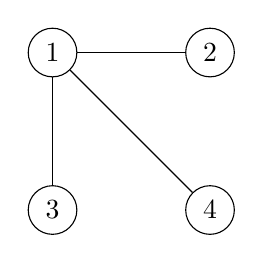
\begin{tikzpicture}
            \node[draw, circle] (A) at (0, 2) {1};
            \node[draw, circle] (B) at (2, 2) {2};
            \node[draw, circle] (C) at (0, 0) {3};
            \node[draw, circle] (D) at (2, 0) {4};

            \draw (A) -- (B);
            \draw (A) -- (C);
            \draw (A) -- (D);
        \end{tikzpicture}
        \captionof{figure}{An example graph} \label{fig:repr:graph1}
    \end{center}
\end{absolutelynopagebreak}

We can represent this graph using the following adjacency matrix:

\begin{absolutelynopagebreak}
    \begin{center}
        $$
            \begin{bytefield}[bitwidth=1.25em]{4}
                \bitheader{0,1,2,3} \\
                \bitboxes{1}{0111} \\
                \bitboxes{1}{1000} \\
                \bitboxes{1}{1000} \\
                \bitboxes{1}{1000} \\
            \end{bytefield}
        $$
        \captionof{figure}{The adjacency matrix of the graph in (\ref{fig:repr:graph1})}
        \label{fig:repr:adjmatrix1}
    \end{center}
\end{absolutelynopagebreak}

Using this representation we can easily check if two vertices are connected ($O(1)$) but we need a lot of space to store it ($O(|V|^2)$).

Adjacency matrices can be useful can be useful since we can perform linear algebra magic on them
(e.g.: compute the $k$ power, or find the eigenvalues) to find some properties of the graph.

\subsubsection{Adjacency list}

This is a more space efficient way to represent a graph, especially if the graph is sparse (meaning it has few edges and a lot of nodes).

\begin{bluebox}{Definition}
    Let $G = (V, E)$ be a graph with $|V| = n$.

    An \textbf{adjacency list} is a list of $n$ lists where the $i$-th list contains all the vertices adjacent to the $i$-th vertex.
\end{bluebox}

\textbf{Example}: The graph in (\ref{fig:repr:graph1}) can be represented using the following adjacency list:

\begin{absolutelynopagebreak}
    \begin{center}
        \begin{tabular}{c|c}
            Vertex & Adjacent vertices \\
            \hline
            1      & 2, 3, 4           \\
            2      & 1                 \\
            3      & 1                 \\
            4      & 1
        \end{tabular}
        \captionof{figure}{The adjacency list of the graph in (\ref{fig:repr:graph1})}
        \label{fig:repr:adjlist1}
    \end{center}
\end{absolutelynopagebreak}

This in practice can be implemented using linked lists: in this case we have a space complexity of $O(|V| + |E|)$ while the time complexity to find if a vertex is connected to another one is $O(|E|)$.

(Is really linked lists the best way to implement this? What about other data structures?)

\subsubsection{Summerizing}

We can use the following table to summarize the two representations:

\begin{center}
    \begin{tabular}{c|c|c|c}
               & space          & $(u, v) \in E$ & all neighbors \\
        \hline
        matrix & $O(|V|^2)$     & $O(1)$         & $O(|V|)$      \\
        list   & $O(|V| + |E|)$ & $O(d(v))$      & $O(d(v))$
    \end{tabular}
    \captionof{table}{Comparison of graph representations}
    \label{tab:graphrepr}
\end{center}

\subsection{Exploring a graph - Depth First Search (DFS)}

In this section we will look at algorithms to explore a graph.

We setup the algorithm like this:

\begin{minted}{python}
    # These are the variables we will be using:
    clock = 1
    visited = {}
    pre = {}
    post = {}

    def setup(G):
        clock = 1
        for v in G.vertices():
            visited[v] = False
            pre[v] = None  # time of first visit of `v`
            post[v] = None # time of last visit of `v`
\end{minted}

The actual algorithm is as follows:

\begin{minted}{python}
    def explore(G, v):
        visited[v] = True
        pre[v] = clock
        clock += 1
        for (u, v) in v.edges():
            if not visited[u]:
                explore(G, u)
        post[v] = clock
        clock += 1
\end{minted}

Then we call \texttt{explore} on any vertex of $G$ and let the function traverse the graph.

\section{Class of 14/02/2024 - DFS continued}

\subsection{Formal statement}

We can now state the algorithm formally:

\underline{Statement}: Let $G = (V, E)$ be a graph and $v \in V$.
The algorithm \texttt{explore(G, v)} visits all the vertices of $G$ that are reachable from $v$.

This is equivalent to

\underline{Statement}: $v$ can reach $u$ $\iff$ \texttt{visited[u]} is \texttt{True} after completing \texttt{explore(G, v)}.

\begin{proof}
    We prove each implication separately:

    \begin{description}
        \item[$\impliedby$] Since we started from \texttt{visited} containing only \texttt{False} values,
            the only way \texttt{visited[u]} can be \texttt{True} is if $u$ was part of the exploration of some other node $w$.
            If $W = v$ we are done, otherwise we can repeat the argument for $w$.
            We know this procedure will terminate since the graph is finite.
        \item[$\implies$] We prove this by contradiction.
            Suppose that $u$ is reachable from $v$ and that there is a run of \texttt{explore} that misses $u$.
            Since $u$ is reachable from $v$ there is a path from $v$ to $u$.
            Let $w$ be the first vertex on this path that is not visited by the run of \texttt{explore} and let $z$ be the vertex that precedes $w$.
            This is a contradiction, by the way the algorithm is defined, since $w$ is a neighbor of $z$ and it is not visited we visit it.
    \end{description}
\end{proof}

By the definition of the algorithm we have that it doesn't work if we have a graph with more than 1 connected component.

We can complete the algorithm to take care of this case too:

\begin{minted}{python}
    def DFS(G):
        # Setup
        clock = 1
        visited = {}
        pre = {}
        post = {}

        for v in G.vertices():
            visited[v] = False
            pre[v] = None
            post[v] = None

        # Run the algorithm for all nodes.
        # This will actually call `explore` just once
        # per connected component.
        for v in G.vertices():
            if not visited[v]:
                explore(G, v)

\end{minted}

\subsection{Time complexity}

We have that the setup part is $O(|V|)$, since we are looping through all nodes.

For the actual \texttt{explore} part we have at least $O(|V|)$ since for each node we have to set \texttt{visited} to \texttt{True},
but we have to take in account the time to visit all the edges of the graph:
each edge is visited exactly twice.

Combining the two parts we have that the time complexity of the algorithm is $O(|V| + |E|)$.

\subsection{About the pre and post variables}

\underline{Remark}: For every node $v$ we have that \texttt{pre[v]} $<$ \texttt{post[v]}.

\begin{proof}
    This is obvious from the definition of the algorithm.
\end{proof}

\underline{Theorem}: For every node $v$ and $u$, the intervals $[\text{pre}(v), \text{post}(v)]$ and $[\text{pre}(u), \text{post}(u)]$ are either disjoint or one is contained in the other.

\begin{proof}
    We have two cases:
    \begin{enumerate}
        \item $\text{pre}(v) < \text{post}(u)$, hence $\text{pre}(u) < \text{pre}(v) < \text{post}(u)$. This means that $v$ is a descendant of $u$, thus the exploration of $v$ must have ended before the exploration of $u$.
              We have that $\text{pre}(u) < \text{pre}(v) < \text{pre}(u) < \text{post}(v)$, hence the intervals are contained in one another.
        \item $\text{pre}(u) > \text{post}(v)$, hence $\text{pre}(u) < \text{post}(u) < \text{pre}(v) < \text{post}(v)$ and the intervals are disjoint.
    \end{enumerate}
\end{proof}

\subsection{Counting connected components}

We can modify the algorithm to count the number of connected components in the graph.

\begin{minted}{python}
    def DFS(G):
        clock = 1
        visited = {}
        pre = {}
        post = {}
        cc = {}

        for v in G.vertices():
            visited[v] = False
            pre[v] = None
            post[v] = None
            cc[v] = None

        connected_component = 0

        for v in G.vertices():
            if not visited[v]:
                connected_component += 1
                explore(G, v)


    def explore(G, v):
        cc[v] = connected_component
        # The rest of the algorithm is the same


\end{minted}

In this way, at the end of the procedure the variable \texttt{connected\_component} will contain the number of connected components in the graph
and the variable \texttt{cc} will contain the connected component of each node.

\section{Class of 15/02/2024 - DFS continued}

\subsection{DFS-Tree}

We can introduce a new variable, initialized as

\begin{minted}{python}
    parent = {}
    for v in G.vertices():
        parent[v] = None
\end{minted}

When exploring the graph we set this variable to the node that called the current one.
In this way we can build a tree that represents the exploration of the graph.

\subsection{Directed graphs}

\begin{center}
    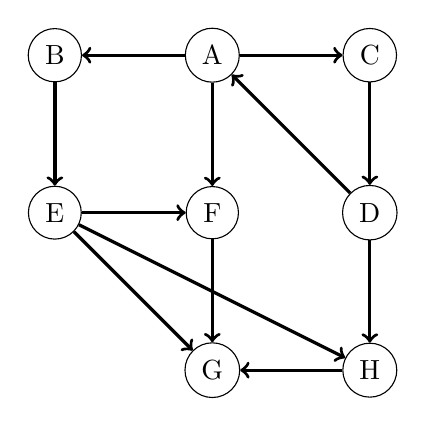
\begin{tikzpicture}
        \node[draw, circle] (A) at (0, 0) {A};
        \node[draw, circle] (B) at (-2, 0) {B};
        \node[draw, circle] (C) at (2, 0) {C};
        \node[draw, circle] (D) at (2, -2) {D};
        \node[draw, circle] (E) at (-2, -2) {E};
        \node[draw, circle] (F) at (0, -2) {F};
        \node[draw, circle] (G) at (0, -4) {G};
        \node[draw, circle] (H) at (2, -4) {H};

        \draw[->, very thick] (A) -- (B);
        \draw[->, very thick] (A) -- (C);
        \draw[->, very thick] (C) -- (D);
        \draw[->, very thick] (D) -- (A);
        \draw[->, very thick] (A) -- (F);
        \draw[->, very thick] (B) -- (E);
        \draw[->, very thick] (E) -- (F);
        \draw[->, very thick] (E) -- (G);
        \draw[->, very thick] (E) -- (H);
        \draw[->, very thick] (D) -- (H);
        \draw[->, very thick] (F) -- (G);
        \draw[->, very thick] (H) -- (G);
    \end{tikzpicture}
    \captionof{figure}{An example of a directed graph} \label{fig:directedgraph}
\end{center}

By looking at the graph in (\ref{fig:directedgraph}) and performing a DFS in our head we can see that, starting from $A$, we can reach all the other nodes.
We also note that this is not true for every node, for example $G$ cannot reach any other node.

If we construct the DFS tree of this graph starting from $A$ and breaking ties in alphabetical order we get the following tree:

\begin{center}
    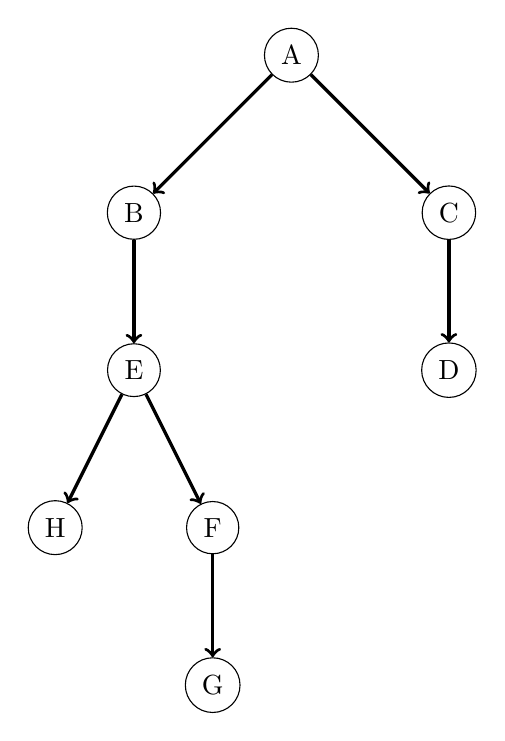
\begin{tikzpicture}
        \node[draw, circle] (A) at (0, 0) {A};
        \node[draw, circle] (B) at (-2, -2) {B};
        \node[draw, circle] (C) at (2, -2) {C};
        \node[draw, circle] (D) at (2, -4) {D};
        \node[draw, circle] (E) at (-2, -4) {E};
        \node[draw, circle] (F) at (-1, -6) {F};
        \node[draw, circle] (G) at (-1, -8) {G};
        \node[draw, circle] (H) at (-3, -6) {H};

        \draw[->, very thick] (A) -- (B);
        \draw[->, very thick] (A) -- (C);
        \draw[->, very thick] (C) -- (D);
        \draw[->, very thick] (B) -- (E);
        \draw[->, very thick] (E) -- (F);
        \draw[->, very thick] (F) -- (G);
        \draw[->, very thick] (E) -- (H);
    \end{tikzpicture}
    \captionof{figure}{The DFS tree of the graph in (\ref{fig:directedgraph})} \label{fig:dfs-tree}
\end{center}

We can define the following for DFS trees:

\begin{description}
    \item[Forward edge] an edge of the original graph that goes from a node to one of its descendants in the DFS tree.
    \item[Back edge] an edge of the original graph that goes from a node to one of its ancestors in the DFS tree.
    \item[Cross edge] an edge of the original graph that goes from a node to a node that is neither an ancestor nor a descendant.
\end{description}

\begin{center}
    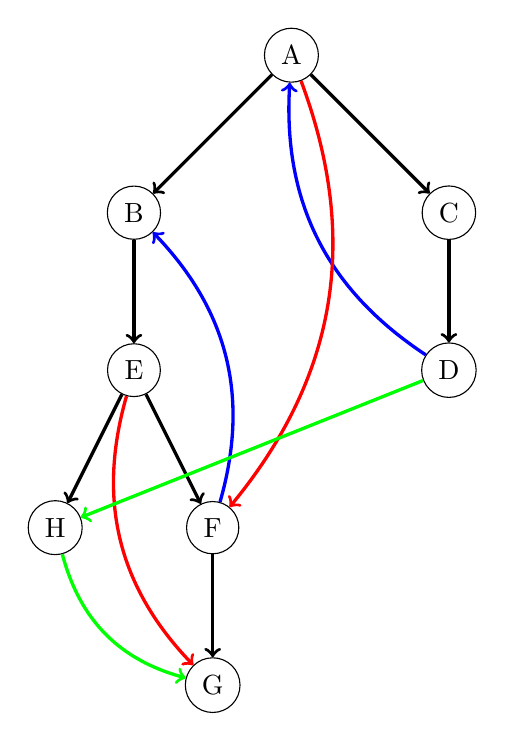
\begin{tikzpicture}
        \node[draw, circle] (A) at (0, 0) {A};
        \node[draw, circle] (B) at (-2, -2) {B};
        \node[draw, circle] (C) at (2, -2) {C};
        \node[draw, circle] (D) at (2, -4) {D};
        \node[draw, circle] (E) at (-2, -4) {E};
        \node[draw, circle] (F) at (-1, -6) {F};
        \node[draw, circle] (G) at (-1, -8) {G};
        \node[draw, circle] (H) at (-3, -6) {H};

        \draw[->, very thick] (A) -- (B);
        \draw[->, very thick] (A) -- (C);
        \draw[->, very thick] (C) -- (D);
        \draw[->, very thick] (B) -- (E);
        \draw[->, very thick] (E) -- (F);
        \draw[->, very thick] (F) -- (G);
        \draw[->, very thick] (E) -- (H);

        % Back edges
        \draw[->, very thick, blue] (D) to [bend left] (A);
        \draw[->, very thick, blue] (F) to [bend right] (B);

        % Forward edges
        \draw[->, very thick, red] (A) to [bend left] (F);
        \draw[->, very thick, red] (E) to [bend right] (G);

        % Cross edges
        \draw[->, very thick, green] (D) to (H);
        \draw[->, very thick, green] (H) to [bend right] (G);

    \end{tikzpicture}
    \captionof{figure}{The DFS tree of the graph in (\ref{fig:directedgraph}) with forward (red), back (blue), and cross edges (green)} \label{fig:dfs-tree-fbg}
\end{center}

We note that if we consider the pre and post variable for each node as an \say{interval},
we can see that nodes connected with a forward edge have the interval of the children contained into the interval of the parent,
nodes connected with a back edge have the interval of the parent contained in the interval of the children,
and nodes connected with a cross edge have disjoint intervals.

\subsection{Theorems about edges}

\subsubsection{Edges in undirected graphs}

\underline{Statement}: In a DFS of an undirected graph, every edge is either a tree edge or a back edge.

\begin{proof}
    Let $\{u, v\}$ be an edge of $G$ and suppose that $\text{pre}(u) < \text{pre}(v)$, hence $u$ is discovered before $v$.

    We have two cases:

    \begin{itemize}
        \item If the first time the search explores $\{u, v\}$ is in the direction from $u$ to $v$ then $v$ is undiscovered until that time.
              Then the edge $\{u, v\}$ is a tree edge.
        \item If the first time the search explores $\{u, v\}$ is in the direction from $v$ to $u$ then $v$ is already discovered.
              Then the edge $\{u, v\}$ is a back edge.
    \end{itemize}
\end{proof}

\subsubsection{Cycles and back edges}

\underline{Statement}: A directed graph has a cycle $\iff$ a DFS of the graph has at least one back edge.

\begin{proof}
    We prove each implication separately:

    \begin{description}
        \item[$\impliedby$] If $(u, v)$ is a back edge then there is a cycle consisting of the edge $(u, v)$ and the path from $v$ to $u$ in the DFS tree. We know such path exists since to have a back edge we have to get to $v$ with $u$ already being discovered.
        \item[$\implies$] If $G$ has a cycle, then we can write it as $v_0 \to v_1 \to \dots \to v_k \to v_0$.
            Let $v_i$ be the first vertex in the cycle that is discovered.
            When we enter the cycle all the other nodes of the cycle are undiscovered since $v_i$ is the first one by definition. Since DFS visits all the \say{legal} edges the algorithm will visit all edges of the cycle, hence eventually it will reach the edge $(v_{i-1}, v_i)$, which is a back edge.
    \end{description}
\end{proof}

\subsection{Topological Sort}

\underline{Definition}: If $G = (V, E)$ is a directed graph we say that an ordered list $L$ of the vertices in $V$ is a \textbf{topological sort} of $G$ if for every edge $(u, v) \in E$, the vertex $u$ comes before $v$ in $L$.

\underline{Example}: Consider the graph in Figure (\ref{fig:directedgraph}). A topological sort of this graph is $[A, C, D, B, E, F, H, G]$.
Note that topological sorts are not unique.

\section{Class of 16/02/2024 - Topological sort continued}

\subsection{Cycles and topological sorts}

\subsubsection{Theorem: cycle implies no topological sort}

\underline{Statement}: If a directed graph has a cycle then it has no topological sorts.

\begin{proof}
    By contradiction, we assume that $G$ has a topological sort $L$.
    Let $v_0, v_1, \dots, v_k$ be the cycle in $G$.
    Every node $v_i$ in the cycle has a predecessor $u$, such that $(v_i, u) \in E$.
    Let $\overline{v}$ be the first node in the cycle that is in $L$.
    Since $\overline {u}$ is a predecessor of $\overline{v}$, $\overline{u}$ comes before $\overline{v}$ in $L$,
    but this is a contradiction since $\overline{v}$ comes before $\overline{u}$ in the cycle.
\end{proof}

\subsubsection{Lemma: incoming edges and cycles}

\underline{Statement}: If $G = (V, E)$ is a directed graph in which every vertex has at least one incoming edge, then $G$ has at least one cycle.

\begin{proof}
    Take any vertex $v$ in $V$ and call it $v_{n+1}$, where $n = |V|$.

    Since every vertex has at least one incoming edge, there exists a vertex $v_n$ such that $(x, v_{n+1}) \in E$.

    We repeat this process until we reach a vertex $v_1$, which will have an outgoing edge to some other vertex $\overline{v}$ that we have already visited.
\end{proof}

\subsubsection{Theorem: no cycle implies topological sort}

\underline{Statement}: If a directed graph $G$ doesn't contain a cycle,
then it has at least one topological sort.

\begin{proof}
    We will prove this by constructing an algorithm that will find a topological sort of $G$.

    \begin{minted}{python}
        def find_topological_sort(G):
            L = []
            V = G.vertices()
            E = G.edges()
            while len(V) > 0:
                v = V.get_vertex_with_no_incoming_edges()
                L.append(v)
                V.remove(v)
                E.remove_all_edges_from(v)
            return L
    \end{minted}

    The idea is that if a vertex has no incoming edges then it is correct to append it to the list.

    This algorithm will work since we will always be able to get a vertex with no incoming edges since, if we couldn't, we would have a cycle (by the lemma above).

\end{proof}

\subsection{Topological sorts from DFS}

\subsubsection{Theorem: DFS and topological sorts in DAGs}

Consider the following the following algorithm:

\begin{minted}{python}
    visited = {}
    L = []

    def explore(G,v):
        visited[v] = True
        for (u, v) in v.edges():
            if not visited[u]:
                explore(G, u)
        L.append(v)
\end{minted}

We want to prove that the list $L$ will be a topological sort of the graph $G$ by the end of the algorithm.

Now we formally state and prove this.

\underline{Statement}: $G=(V, E)$ is a directed acyclic graph (DAG). If we run the algorithm \texttt{DFS(G)}, then for every edge $(u, v) \in E$, the call to \texttt{explore(G, u)} will end after the call to \texttt{explore(G, v)}.

\begin{proof}
    We look at the state of the algorithm when the edge $(u, v)$ is explored.
    The other vertices can be in one of the following states:
    \begin{enumerate}
        \item not yet visited
        \item visited and in \texttt{L}
        \item visited but not in \texttt{L} because the exploration of the vertex has not ended yet
    \end{enumerate}

    We note that when we explore $u$, $v$ will be in state 1 or 2, not 3.
    This is because if $v$ is in state 3 then there exist a path from $v$ to $u$ and we have a cycle, which is a contradiction.

    Now we consider the two possible cases separately:
    \begin{enumerate}
        \item Then we are about to explore from $u$. $v$ is a neighbor of $u$ and it is unexplored yet so we will explore it.
              The exploration of $v$ will end before the exploration of $u$.
        \item Then the exploration of $v$ has already ended. This means that the exploration of $u$ will end after the exploration of $v$.
    \end{enumerate}

    In both cases we have our result.
\end{proof}

This theorem works for any DAG, but not any directed graph is a DAG.

\subsection{Strongly connected components (SCC)}

\subsubsection{Reverse of a graph}

\underline{Definition}: Given a directed graph $G=(V, E)$,
the \textbf{reverse} of $G$ is the graph $G^R = (V, E^R)$ where $(u, v) \in E^R \iff (v,u) \in E$.

\subsubsection{Theorem: component graphs are DAGs}

Let $G$ be a directed graph, then the \textbf{component graph} $G'$ is obtained by grouping all the vertices of a connected components of $G$.

\underline{Statement}: If $G$ is a directed graph and $G'$ is its component graph, then $G'$ is a directed acyclic graph.

\begin{proof}
    We prove this by contradiction.

    Suppose that $G'$ has a cycle $C_1, \ldots, C_n$.
    This means that it is possible for any $v \in C_i$ to reach any $u \in C_{i+1}$.
    This means that the two components should be merged, which is a contradiction.
\end{proof}

\subsubsection{Theorem: strongly connected components in the reverse}

\underline{Statement}: Let $G = (V, E)$ be a directed graph and $G^R = (V, E^R)$ its reverse.
Then the connected components of $G^R$ are the strongly connected components of $G$.

\begin{proof}
    If we consider $G^R$ we have that the connected components stay connected in the reverse, and they don't get connected to other components since $G'$ is a DAG.

    % TODO: ???? is this formal enough?
\end{proof}

\subsubsection{Theorem: post numbers in SCCs}

\underline{Statement}: If $C, C'$ are two strongly connected components (SCC) of a directed graph $G$ and there is an edge from a node in $C$ to a node in $C'$, then the highest \texttt{post} number in $C$ is greater than the highest \texttt{post} number in $C'$.

\begin{proof}
    If DFS visits the component $C$ before $C'$ then all of $C'$ will be visited before we exit $C$.

    If DFS visits $C'$ before $C$ then $C$ will not be visited until we exit $C'$.
\end{proof}

\subsubsection{Definitions: source and sink}

\underline{Definition}:
\begin{itemize}
    \item Source is a vertex with no incoming edges.
    \item Sink is a vertex with no outgoing edges.
\end{itemize}

Note that the source will have the highest \texttt{post} number.

Reversing the graph will transform the sources into sinks and vice versa.

\subsubsection{Finding SCCs}

To find SCCs we can use the following algorithm:

\begin{minted}{python}
    # Consider an explore function that
    # returns a list of the vertices explored

    def find_SCCs(G):
        V = G.vertices()
        SCCs = {}
        while len(V) > 0:
            G_R = G.reverse()
            explored_nodes_of_reverse = explore(G_R, G_R.random_vertex())
            sink = explored_nodes_of_reverse.get_vertex_with_highest_post()

            # These nodes are all part of the same SCC
            explored_nodes = explore(G, sink)
            SCCs.add(explored_nodes)
            V.remove_all(explored_nodes)

    return SCCs
\end{minted}

\section{Class of 21/02/2024 - Shortest path}

\subsection{Introduction}

For this class we had to hand in an assignment,
you can find my solution in \texttt{cs\_assignment\_1.pdf}.

The problem we are going to look at now is how to get from one vertex to another in a graph passing through the fewest number of edges.

It's easy to see that DFS is not the right tool for this problem. We need to find a different algorithm.

\textbf{\underline{Definition} (shortest path)}:
Let $G = (V, E)$ and $s \in V$ be the start vertex.
The shortest path distance $d(v)$ from $s$ to $v \in V$ is the minimum number of edges in any path from $s$ to $v$.
If there is no path from $s$ to $v$ then $d(v) = \infty$.

\subsection{Breadth First Search (BFS)}

This is the algorithm we will use to find the shortest path.

It works in the following way:

\begin{minted}{python}
    def BFS(G, s):
        distance = {}
        for v in G.vertices():
            distance[v] = float('inf')

        distance[s] = 0
        queue = Queue()
        queue.enqueue(s)

        while not queue.is_empty():
            v = queue.dequeue()
            for u in v.neighbors():
                if distance[u] == float('inf'):
                    distance[u] = distance[v] + 1
                    queue.enqueue(u)
\end{minted}

You can watch the algorithm in action here: \url{https://www.cs.usfca.edu/~galles/visualization/BFS.html}.

\subsubsection{Sidenote: queues}

For this algorithm we use a \texttt{Queue} data structure.

Queues are similar to arrays and have the following operations:
\begin{itemize}
    \item \texttt{enqueue(x)}: add an element to the end of the queue
    \item \texttt{dequeue()}: remove the first element of the queue and returns it
\end{itemize}

Sometimes \texttt{enqueue} is called \texttt{inject} and \texttt{dequeue} is called \texttt{eject}.

We say that queues are \textit{FIFO} (First In First Out) data structures.

\subsubsection{Proof of correctness}

\textbf{\underline{Theorem} (correctness of BFS)}: Let $G = (V, E)$ be a graph and $s \in V$.
Assume the range of distances $d$ from $s$ to all other vertices is $[0, M]$.
For each $t \in [0, M]$ there is an iteration of the algorithm such that:
\begin{enumerate}
    \item all the vertices $v \in \texttt{queue}$ have $d[v] = t$
    \item all the vertices $u$ that have been removed from \texttt{queue} have $d[u]$ equal to the correct distance from $s$ to $u$
    \item For all vertices $u$ that have been removed from \texttt{queue} we have that $d[u] \leq t - 1$
\end{enumerate}

Note that since the conditions (1), (2), and (3) have to be true for any $t$ we call them \textit{invariants}.

\begin{proof}
    We will prove this by induction on $t$.

    \begin{description}
        \item[Base case] $t = 0$.
            This is trivially true since the only vertex in the queue is $s$ and $d[s] = 0$.

        \item[Inductive step] We assume that the statements are true for $t = \tau$.

            At this time, some vertices have been already removed from \texttt{queue}, others are still in it, and some have yet to be explored.

            At this point of time we know the following facts:
            \begin{itemize}
                \item By (3), all vertices removed from \texttt{queue} have $d[u] \leq \tau - 1$
                \item By (2) the distances are correct.
                \item By (1), all vertices in \texttt{queue} have $d[v] = \tau$.
            \end{itemize}

            At the next round $\tau + 1$, BFS will go through as many iterations as the number of vertices in \texttt{queue}: the algorithm will remove those vertices.
            Note that these vertices vertices have all distance $\tau$ and their distance is no longer going to change. This implies that (2) and (3) are true.

            Moreover, all vertices not yet seen that are neighbor of the ones that were in \texttt{queue} at $\tau$ have their distances set to $\tau + 1$, thus (1) is true.
    \end{description}
\end{proof}

\subsubsection{Time complexity}

We split the algorithm in parts:

\begin{itemize}
    \item The setup part of the algorithm is $O(|V|)$.
    \item We check whether the queue is empty $|V| + 1$ times, hence $O(|V|)$.
    \item We insert a vertex in the queue based on its neighbors, hence $O(|E|)$.
    \item We enqueue and dequeue every vertex in the graph at most once, hence $O(|V|)$.
\end{itemize}

Combining all the steps we get a time complexity of $O(|V| + |E|)$.

Note that we need to take in account the time for queue operations, which depend on the implementation of the queue itself.

\subsubsection{Time complexity of queue operations - basic}

For the sake of this course its enough to know that queue both \texttt{enqueue} and \texttt{dequeue} are $O(1)$.

Moreover queues are usually implemented using a linked list, but if you know already the maximum size of the queue you can also use an array which is slightly more efficient.

\subsubsection{Implementation of a queue - if you're curious}

\begin{warningbox}{Advanced stuff ahead}
    This is not part of the course, but if you are curious you can read on.

    The following code snippets are written in C.
\end{warningbox}

We will implement a queue using a linked list as underlying data structure.

\begin{minted}{c}
    struct node {
        int data;
        struct node *next;
    };

    struct queue {
        struct node *head;
        struct node *tail;
    };

    struct queue *create_queue() {
        struct queue *q = malloc(sizeof(struct queue));
        q->head = NULL;
        q->tail = NULL;
        return q;
    }

    void enqueue(struct queue *q, int x) {
        struct node *n = malloc(sizeof(struct node));
        n->data = x;
        n->next = NULL;
        if (q->head == NULL) {
            q->head = n;
            q->tail = n;
        } else {
            q->tail->next = n;
            q->tail = n;
        }
    }

    int dequeue(struct queue *q) {
        int x = q->head->data;
        struct node *n = q->head;
        q->head = q->head->next;
        free(n);
        return x;
    }
\end{minted}

We see that each of the operations do not depend on the length of the queue, hence they are both $O(1)$.

Note that in this implementation we have to \texttt{malloc} each node (which is a slow operation) and dereference a pointer (which can also be slow).

If we know the maximum size of the queue we can use an array to implement it, which will make the operations even faster.

The idea is that we keep a pointer of the first and last element of the queue and we use an array to store the elements.

When we enqueue an element we add it to the end of the array and we increment the pointer to the last element.
When we dequeue an element we return the first element of the array and we increment the pointer to the first element.

If we run out of space at the end of the array we can just cycle back to the beginning since, by knowing the maximum size of the queue, we are sure that the first elements are not going to be used anymore at the time we have to cycle back to the start.

\begin{minted}{c}
    struct queue {
        int *data;
        off_t head;
        off_t tail;
        size_t size;
    };

    struct queue *create_queue(size_t size) {
        struct queue *q = malloc(sizeof(struct queue));
        q->data = malloc(size * sizeof(int));
        q->head = 0;
        q->tail = 0;
        q->size = size;
        return q;
    }

    void enqueue(struct queue *q, int x) {
        q->data[q->tail] = x;
        q->tail = (q->tail + 1) % q->size;
    }

    int dequeue(struct queue *q) {
        if (q->head == q->tail) {
            // The queue is empty
            return -1;
        }

        int x = q->data[q->head];
        q->head = (q->head + 1) % q->size;
        return x;
    }
\end{minted}

We see that the operations are still $O(1)$ but this time we \texttt{malloc} only once and we don't have to dereference any pointers.

\section{Class of 22/02/2024 - Dijkstra's algorithm}

We now consider a graph $G = (V, E)$ and a function $l(u, v) > 0$ that assigns a length to each edge $(u, v) \in E$.

Today's problem is to find the shortest path from a vertex $s \in V$ to any other vertex taking into account the length of the edges.

\begin{figure}[H]
    \centering
    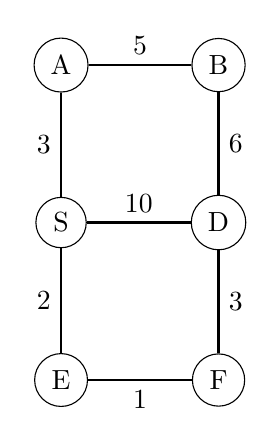
\begin{tikzpicture}
        \node[draw, circle] (A) at (0, 0) {A};
        \node[draw, circle] (B) at (2, 0) {B};
        \node[draw, circle] (S) at (0, -2) {S};
        \node[draw, circle] (D) at (2, -2) {D};
        \node[draw, circle] (E) at (0, -4) {E};
        \node[draw, circle] (F) at (2, -4) {F};

        \draw[thick] (S) -- node[left] {3} (A);
        \draw[thick] (S) -- node[above] {10} (D);
        \draw[thick] (A) -- node[above] {5} (B);
        \draw[thick] (D) -- node[right] {6} (B);
        \draw[thick] (E) -- node[below] {1} (F);
        \draw[thick] (D) -- node[right] {3} (F);
        \draw[thick] (S) -- node[left] {2} (E);

    \end{tikzpicture}

    \caption{An example of a graph with weighted edges} \label{fig:weightedgraph}
\end{figure}

We have seen that BFS does a similar job, but it would work only if all the edges had the same length. We need to find a different algorithm.

\subsubsection{Naive approach}

We can try to convert the problem into a shortest path problem with unweighted edges, which we know already how to solve.

For example, we could add new vertices in between each edge, one for each unit of length of the edge, and then connect them with edges of length 1.

It is easy to show that this approach would work and it would convert the problem into one we already solved but it is also highly inefficient.

\subsection{Tools: priority queues}

For this algorithm we will need a new data structure: the priority queue.

A priority queue works more or less like a normal queue but each element of the queue also has a priority.

When we dequeue an element we get the one with the highest priority first, no matter when it was enqueued.

An example of priority queue in real life is the triage in a hospital: the patients are not treated in the order they arrived but in the order of the severity of their condition.

\subsubsection{Implementation with a linked list}

This is the simplest implementation and the original one that Dijkstra used.

\begin{center}
    \begin{tabular}{|c|c|}
        \hline
        \textbf{Operation}  & \textbf{Time complexity} \\
        \hline
        Init                & $O(n)$                   \\
        Check empty         & $O(1)$                   \\
        Find min and remove & $O(n)$                   \\
        Update priority     & $O(1)$                   \\
        \hline
    \end{tabular}
    \captionof{table}{Time complexity of the operations of a priority queue implemented with a linked list}
    \label{tab:priorityqueue_linkedlist}
\end{center}

Note that these operations have these time complexities only if applied to this specific algorithm, in general they can be different.

\subsubsection{Implementation with a binary heap}

First we need to define a \textit{full binary tree}.

A full binary tree is a rooted tree where each note has two children (left and right) or no children at all, except possibly on the bottom layer.

\begin{figure}[H]
    \centering
    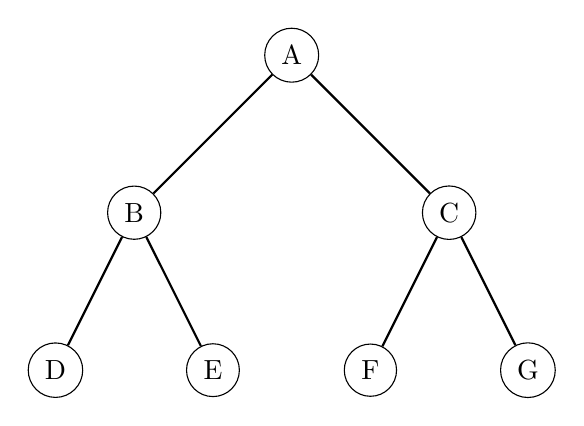
\begin{tikzpicture}
        \node[draw, circle] (A) at (0, 0) {A};
        \node[draw, circle] (B) at (-2, -2) {B};
        \node[draw, circle] (C) at (2, -2) {C};
        \node[draw, circle] (D) at (-3, -4) {D};
        \node[draw, circle] (E) at (-1, -4) {E};
        \node[draw, circle] (F) at (1, -4) {F};
        \node[draw, circle] (G) at (3, -4) {G};

        \draw[thick] (A) -- (B);
        \draw[thick] (A) -- (C);
        \draw[thick] (B) -- (D);
        \draw[thick] (B) -- (E);
        \draw[thick] (C) -- (F);
        \draw[thick] (C) -- (G);
    \end{tikzpicture}
    \caption{An example of a full binary tree} \label{fig:fullbinarytree}
\end{figure}

If the number of nodes is different than $2^h - 1$ for some $h$ then we start filling the tree from the left and we say that the tree is not full.

We can navigate the tree as follows:

\begin{itemize}
    \item From a parent of index $i$ we can get to the left child at index $2i$ and to the right child at index $2i + 1$.
    \item From a child at index $i$ we can get to the parent at index $\lfloor i / 2 \rfloor$.
\end{itemize}

Therefore this data structure can be implemented using an array and navigated using the above formulas.

We can now introduce a minimum binary heap or \textbf{min-heap}:
this is a binary heap where the value of every node is less than or equal to the value of its children.

\begin{figure}[H]
    \centering
    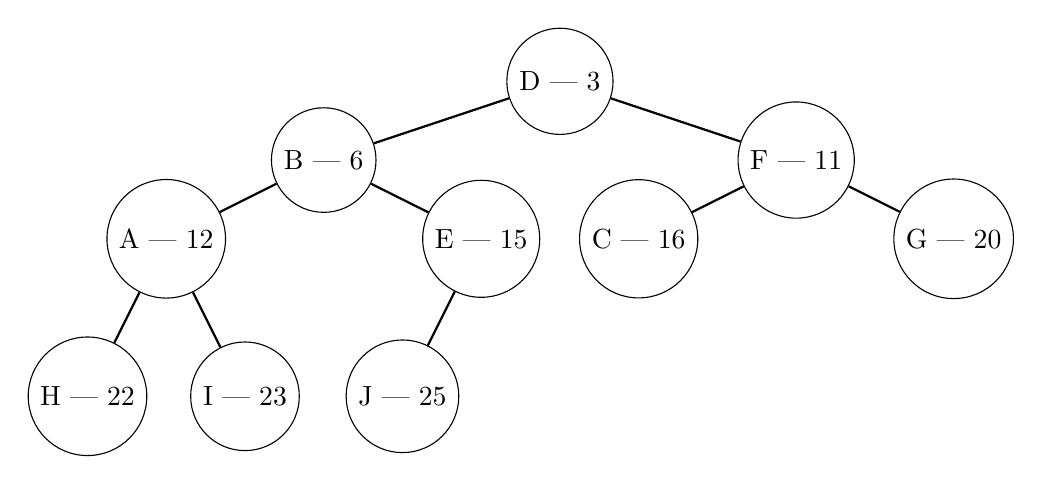
\begin{tikzpicture}
        \node[draw, circle] (D) at (0, -1) {D | 3};
        \node[draw, circle] (B) at (-3, -2) {B | 6};
        \node[draw, circle] (F) at (3, -2) {F | 11};
        \node[draw, circle] (A) at (-5, -3) {A | 12};
        \node[draw, circle] (E) at (-1, -3) {E | 15};
        \node[draw, circle] (C) at (1, -3) {C | 16};
        \node[draw, circle] (G) at (5, -3) {G | 20};
        \node[draw, circle] (H) at (-6, -5) {H | 22};
        \node[draw, circle] (I) at (-4, -5) {I | 23};
        \node[draw, circle] (J) at (-2, -5) {J | 25};

        \draw[thick] (D) -- (B);
        \draw[thick] (D) -- (F);
        \draw[thick] (B) -- (A);
        \draw[thick] (B) -- (E);
        \draw[thick] (F) -- (C);
        \draw[thick] (F) -- (G);
        \draw[thick] (A) -- (H);
        \draw[thick] (A) -- (I);
        \draw[thick] (E) -- (J);
    \end{tikzpicture}

    \caption{An example of a min-heap} \label{fig:minheap}
\end{figure}

where the letter is the value of the node and the number is the priority.

We can now compile a table with the time complexity of each operation of a min-heap.

\begin{center}
    \begin{tabular}{ |c|c|c| }
        \hline
        \textbf{Operation} & \textbf{Time complexity} & \textbf{Comment}                        \\
        \hline
        Init               & $O(n \log n)$            & We need to sort the list first          \\
        Check empty        & $O(1)$                   & We can just check if the array is empty \\
        Remove minimum     & $O(\log n)$              & We remove the root and heapify the tree \\
        Update priority    & $O(\log n)$              & We need to heapify the tree             \\
        \hline
    \end{tabular}
    \captionof{table}{Time complexity of the operations of a min-heap}
    \label{tab:minheap}
\end{center}

\textbf{Heapifying} the tree means to restore the property of the min-heap after we removed the root or updated the priority of a node.

\begin{itemize}
    \item
          When we remove the root we swap it with the last node of the tree, then we swap the new root with its smallest child and we keep doing this until the tree is a min-heap again.
          In this process we are doing $O(\log n)$ operations.
    \item
          When we update a priority we just need to swap the node with its parent until the tree is a min-heap again, which is also $O(\log n)$.
\end{itemize}

\subsection{Dijkstra's algorithm}

\subsubsection{Definition}

Let $G(V, E)$, $s \in V$, and $l(u, v) > 0 \forall (u, v) \in E$. Let $d(v)$ be the length of the shortest path from $s$ to $v$.

\begin{minted}{python}
    def Dijkstra(G, s):
        d = {}

        # Setup
        for v in G.vertices():
            d[v] = float('inf')
        d[s] = 0

        # Insert all vertices in the priority queue
        Q = PriorityQueue(G.vertices())
        while not Q.is_empty():

            # Get the vertex with the smallest distance
            u = Q.dequeue()
            for v in u.neighbors():
                # We check if we can reach v in a shorter path
                if d[v] > d[u] + l(u, v):
                    # If we can, we update the distance of v
                    d[v] = d[u] + l(u, v)

                    # Save the newfound distance of v in the queue
                    # by updating its priority
                    Q.update_priority(v, d[v])
\end{minted}

\subsubsection{Example}

\begin{figure}[H]
    \centering
    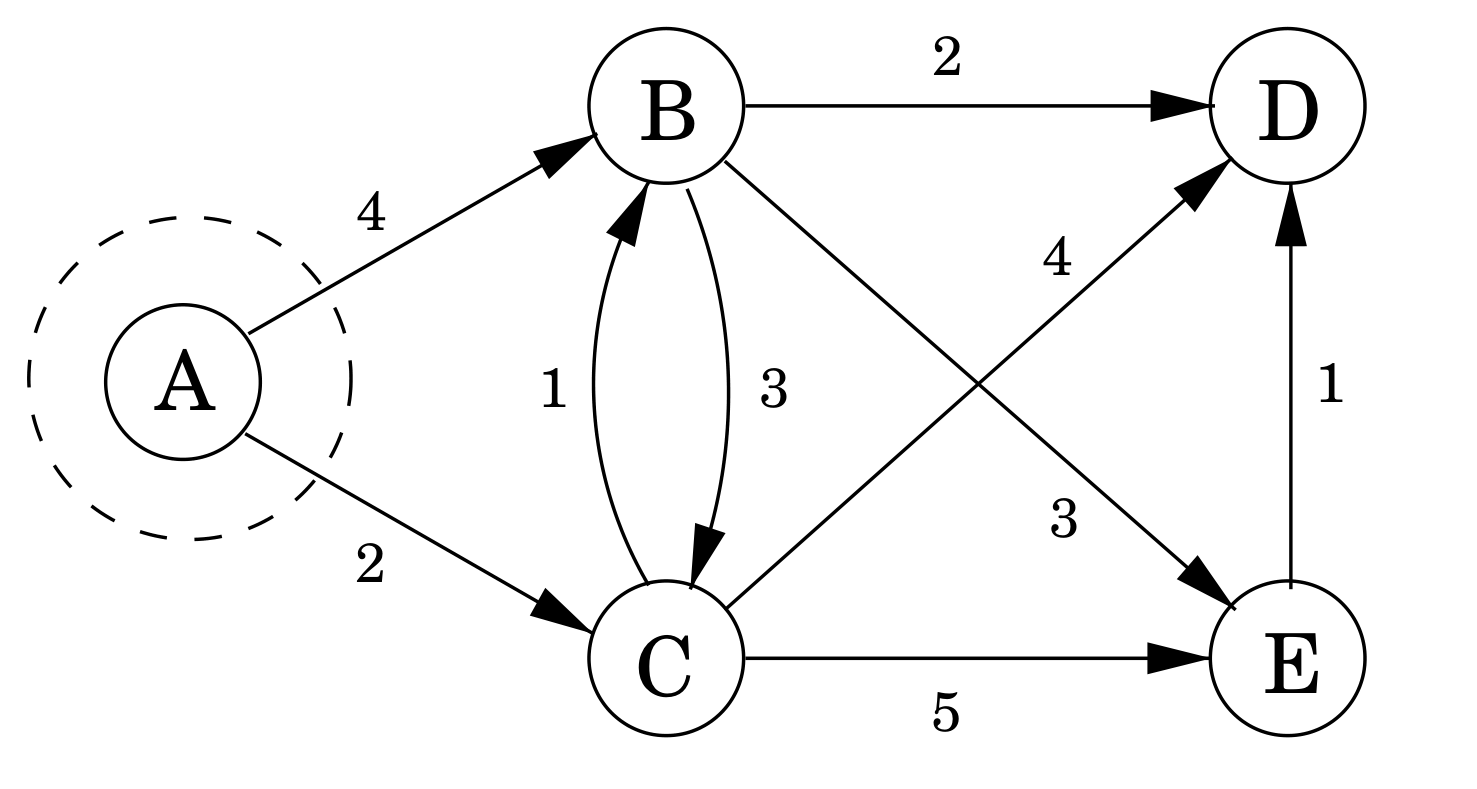
\includegraphics[width=0.4\textwidth]{assets/computer_science_2/dijsktra.png}

    \caption{An example of a directed graph with weighted edges}
    \label{fig:weighted_directedgraph}
\end{figure}

In the graph in Figure (\ref{fig:weighted_directedgraph}) we would start from $A$ which is the start vertex and we apply the algorithm.

We can make a table of the distances at each step of the algorithm:

\begin{center}
    \begin{tabular}{ |c|c|c|c|c|c| }
        \hline
        Extracted vertex & A & B          & C          & D          & E          \\
        \hline
        Setup            & 0 & $\infty$   & $\infty$   & $\infty$   & $\infty$   \\
        A                & 0 & \textbf{4} & \textbf{2} & $\infty$   & $\infty$   \\
        C                & 0 & \textbf{3} & 2          & \textbf{6} & \textbf{7} \\
        B                & 0 & 3          & 2          & \textbf{5} & \textbf{6} \\
        D                & 0 & 3          & 2          & 5          & 6          \\
        E                & 0 & 3          & 2          & 5          & 6          \\
        \hline
    \end{tabular}
    \captionof{table}{The distances at each step of the algorithm}
    \label{tab:dijsktra_distances}
\end{center}

In the Table (\ref{tab:dijsktra_distances}) we have highlighted the vertices that have been updated.

At each step we extract the vertex with the smallest distance from the queue and we update the distances of its neighbors if we can reach them in a shorter path.

\subsubsection{Negative edges}

Sometimes having a negative length edge can be useful, therefore we need to adjust the algorithm to take them into account.

\begin{figure}[H]
    \centering
    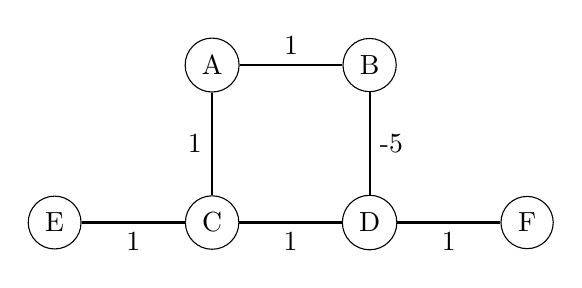
\begin{tikzpicture}
        \node[draw, circle] (A) at (2, 2) {A};
        \node[draw, circle] (B) at (4, 2) {B};
        \node[draw, circle] (C) at (2, 0) {C};
        \node[draw, circle] (D) at (4, 0) {D};
        \node[draw, circle] (E) at (0, 0) {E};
        \node[draw, circle] (F) at (6, 0) {F};

        \draw[thick] (A) -- node[above] {1} (B);
        \draw[thick] (A) -- node[left] {1} (C);
        \draw[thick] (B) -- node[right] {-5} (D);
        \draw[thick] (C) -- node[below] {1} (D);
        \draw[thick] (D) -- node[below] {1} (F);
        \draw[thick] (C) -- node[below] {1} (E);
    \end{tikzpicture}

    \caption{An example of a graph with negative edges}
    \label{fig:negative_edges}
\end{figure}

In the graph in Figure (\ref{fig:negative_edges}) we have a cycle containing a negative edge, which means that we can go around the cycle as many times as we want and we will always decrease the distance.

This is a problem which is not solvable with Dijkstra's algorithm, a graph with \textbf{negative cycles} is not solvable with this algorithm.

Moreover, even if there was no negative cycle but still some negative edges, the algorithm would still not work correctly because it wouldn't be able to find the shortest path.

Despite this flaw we can still use Dijkstra's algorithm in most cases, as long as there are no negative edges.

\subsubsection{Time complexity}

We analyze each step of the algorithm:

\begin{itemize}
    \item The setup part of the algorithm is done once
    \item The check to determine whether the queue is empty is done $|V|$ times
    \item Finding the right vertex to dequeue is done $|V|$ times
    \item Updating the priority of the neighbors of the dequeued vertex is done $|E|$ times
\end{itemize}

Then, we have to take into account the time complexity of the priority queue operations which vary depending on the implementation.

\begin{center}
    \begin{tabular}{ |c|c|c|c|c|c| }
        \hline
        \textbf{Operation}  & \textbf{Times} & \textbf{Linked list} & \textbf{Linked list total} & \textbf{Binary heap} & \textbf{Binary heap total} \\
        \hline
        Init                & 1              & $O(|V|)$             & $O(|V|)$                   & $O(|V| \log |V|)$    & $O(|V| \log |V|)$          \\
        Check empty         & $|V|$          & $O(1)$               & $O(|V|)$                   & $O(1)$               & $O(|V|)$                   \\
        Find min and remove & $|V|$          & $O(|V|)$             & $O(|V|^2)$                 & $O(\log |V|)$        & $O(|V| \log |V|)$          \\
        Update priority     & $|E|$          & $O(1)$               & $O(|E|)$                   & $O(\log |V|)$        & $O(|E| \log |V|)$          \\
        \hline
    \end{tabular}
\end{center}

Summing up the time complexities we find

\begin{itemize}
    \item The linked list implementation has a total time complexity of $O(|V| + |V|^2 + |E|)$
    \item The binary heap implementation has a total time complexity of $O(|V| \log |V| + |E| \log |V|)$.
\end{itemize}

\subsubsection{Proof of correctness}

To make the proof easier we will use the following definitions:
\begin{itemize}
    \item At the end of each while loop, the nodes that have been removed from $Q$ are \textit{black}, and the nodes still in $Q$ are \textit{white}.
    \item An \textit{all-black} path from $s$ to $v$ is a path where each node, except possibly $v$, is black.
\end{itemize}

\textbf{\underline{Statement}}: the following invariants hold:

\begin{enumerate}[label=\roman*]
    \item All the black nodes $v$ have a $d(v)$ equal to the length of the shortest path from $s$ to $v$ or $\infty$ if such path does not exist.
    \item All nodes $v$ have $d(v)$ equal to the length of the shortest \textit{all-black} path from $s$ to $v$ or $\infty$ if such path does not exist.
\end{enumerate}

Moreover, at the end of the execution, all nodes are black, and the invariants imply that $d(v)$ is the length of the shortest path from $s$ to $v$ for all $v \in V$, that is, the algorithm is correct.

\begin{proof}
    Before we start we make the following observations:
    \begin{itemize}
        \item At all the times $\forall v \in V$ if $d(v)$ is not $\infty$ then there is an all-black path from $s$ to $v$ of length $d(v)$.
        \item $\forall v \in V$, $d(v)$ is the only decreased from step to step.
        \item If at some point $d(v)$ equals to the length of the shortest path from $s$ to $v$ then $d(v)$ will never change again.
    \end{itemize}
    These are all obvious just by looking at the code.

    Then, we proceed by induction on the number of iterations of the while loop $t$.

    \begin{description}
        \item[Base case]
            At the beginning of the algorithm, $s$ is the only black node and $d(s) = 0$.

            Indeed the shortest path from $s$ to $s$ is of length 0, therefore (i) is true.
            Moreover, for all $v \in V$ if $v = s$ then $d(v) = 0$ and (ii) is true; if $v \neq s$ then either it is a neighbor of $s$ and $d(v) = l(s, v)$ or $d(v) = \infty$ which is again correct.

        \item[Inductive step 1]
            In this step we assume that (i), (ii) are true at $t$ and we want to show that (i) at $t+1$.
            Let $v$ be the vertex that is removed from the queue during the $t+1$-th iteration. We need to argue that $d(v)$ is the length of the shortest path from $s$ to $v$.

            Notice that the algorithm does not  change $d(v)$ after $v$ is removed from the queue, therefore we just need to show that at time $t$ $d(v)$ is the length of the shortest path from $s$ to $v$.

            We argue by contradiction: suppose that at time $t$ there exists a path from $s$ to $v$ of length $L < d(v)$. By (ii) this path must contain a white vertex, let $u$ be the first white vertex along such path. Then, the length of this path up to $u$ is $\geq d(u)$ since (ii) guarantees that $d(u)$ is the shortest path from $s$ to $u$.
            Moreover the length of this path up to $u$ is $\leq L$ since $u$ is a vertex along that path.
            Combining all these facts we get

            $$
                d(u) \leq L < d(v)
            $$

            which is a contradiction of the algorithm itself, since $v$ was chosen to be the white vertex with the smallest $d(.)$ at the end of the $t$-th iteration.

        \item[Inductive step 2] To be explained in the next class.
    \end{description}
\end{proof}

\end{document}